\begin{frame}{Un sondage \gloss{A survey}}
  \begin{columns}
    \column{0.5\textwidth}
      \small
      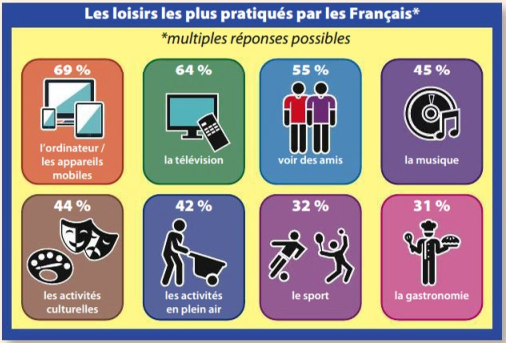
\includegraphics[scale=0.45]{loisirs_france.png} \\
      Les Français... \tinygloss{The French...}
      \begin{itemize}
        \item travaillent 35 heures par semaine. \tinygloss{work 35 hours per week.}
        \item prennent 5 semaines de vacances par année. \tinygloss{take 5 weeks of vacation per year.}
      \end{itemize}
    \column{0.5\textwidth}
      \small
      \begin{minipage}[t][0.8\textheight]{\linewidth}
      Comparons les Français avec la classe.
      En groupes de 5... \\
      \tinygloss{Let's compare the French with the class.
      In groups of 5...}
      \only<1>{
        \begin{enumerate}
          \item Demandez $\to$ \emph{Qui fait (du sport/de la musique/etc)?}
          \item[] \tinygloss{Ask $\to$ \emph{Who does (sports/music/etc)?}}
          \item Comptez les personnes
          \item[] \tinygloss{Count the people}
          \item Écrivez les résultats
          \item[] \tinygloss{Write the results}
        \end{enumerate}
      }
      \only<2>{
        \begin{enumerate}
          \item Annoncez les résultats $\to$ \emph{3 étudiants font du sport dans notre groupe.}
          \item[] \tinygloss{Announce your results $\to$ \emph{3 students do sports in our group.}}
          \item Un/e volontaire écrit le nombres sur le tableau
          \item[] \tinygloss{One volunteer writes the numbers on the board}
          \item Nous faisons les calculs pour le pourcentage de la classe
          \item[] \tinygloss{We calculate the percentage of the class}
        \end{enumerate}
      }
      \end{minipage}
  \end{columns}
\end{frame}